\documentclass[11pt]{article}
\usepackage[width=7.0in, height=10.0in]{geometry}
\usepackage{hyperref}
\usepackage{amsmath}
\usepackage{upgreek}
\usepackage{bm}
\usepackage{mathtools}
\usepackage{tikz}
\usetikzlibrary{arrows}



\newcommand{\vct}[1]{\boldsymbol{\mathbf{#1}}}
\newcommand{\vr}{\vct{r}}
\newcommand{\vrN}{\vr^N}
\newcommand{\vrn}{\vr^n}
\newcommand{\dvr}{\frac{ d \vr  }{(2\pi)^3}}
\newcommand{\vx}{\vct{x}}
\newcommand{\vxN}{\vx^N}
\newcommand{\vxn}{\vx^n}
\newcommand{\dvx}{\frac{ d \vx  }{(2\pi)^3}}
\newcommand{\vk}{\vct{k}}
\newcommand{\dvk}{\frac{ d \vk  }{(2\pi)^3}}
\newcommand{\vy}{\vct{y}}
\newcommand{\vz}{\vct{z}}
\newcommand{\vE}{\vct{E}}
\newcommand{\vD}{\vct{D}}
\newcommand{\vP}{\vct{P}}
\newcommand{\vM}{\vct{M}}
\newcommand{\vMbar}{\overline{\vct{M}}}
\newcommand{\vdel}{\vct{\updelta}}
\newcommand{\vmu}{\vct{\upmu}}

\renewcommand{\theequation}{\thesection.\arabic{equation}}



\begin{document}


\title{Kirkwood's formula for the dielectric constant}
\author{ \vspace{-10ex} }
\date{ \vspace{-10ex} }
\maketitle


This note tries to explain the Kirkwood's 1939 paper\cite{kirkwood1939a}
on the dielectric constant.
%
%We try to use as basic mathematics
%(and to avoid the Legendre polynomials when possible).
Before reading this original paper or the note,
%
the reader is encourage to review Feynman's Lectures on Physics,
Vol. II Chapters 10 and 11.
%
We will use the SI units throughout.
If the reader who prefers the Gaussian units
should simply replace $\epsilon_0$ by $1/(4 \pi)$,
and ignore $4\pi \epsilon_0$ wherever it occurs.



\section{Warm-up models}



First, we recall that the Maxwell equations governing electrostatics
are linear with respect to the fields,
such as the electric field $\vE$ and the charge density $\rho$.
%
This simple fact is very useful,
for it allows us to build up a complex field
by linearly combining simpler electric fields.

In this section,
we will study a few basic model of polarization.
%
These models will be used as building blocks
to understand the more complex Kirkwood model for
the dielectric constant.



\subsection{Uniformly polarized ball}



The effect of a uniformly polarized ball of radius $R$ is equivalent to
that of a uniformly and positively charged ball
located at $\vct c_+ = (0, 0, \delta/2)$ (with charge density $\rho$)
and that of a uniformly and negatively charged ball
located at $\vct c_- = (0, 0, -\delta/2)$,
with $\delta \rightarrow 0$.


The electric field caused by the positive ball
can be computed using the Gauss theorem.
%
For $r_+ < R$, we have
\[
  E 4 \pi r_+^2
=
  \frac { 4 \pi r_+^3 } { 3 } \frac{ \rho } { \epsilon_0 },
\]
where
\[
  r_\pm = |\vr - \vct c_\pm| = r \mp \frac{ \delta \cos\theta} { 2 },
\]
with $\theta$ being the angle between $\vr$ and $\vz$,
i.e., $\hat\vr \cdot \hat\vz = \cos\theta$.
So
\[
  \vE_+
=
  \frac{ \rho } { 3 \, \epsilon_0 } ( \vr - \vct c_+ ).
\]
By symmetry the field caused by the negatively charged ball
is given by
\[
  \vE_- = -\frac{ \rho } { 3 \, \epsilon_0 } ( \vr - \vct c_- ).
\]
The superposition of the two yields
\begin{align}
  \vE_{\vP} = \vE_+ + \vE_-
= - \frac{ \rho \, \vdel } { 3 \epsilon_0 }
= - \frac{ \vP } { 3 \epsilon_0 }
= - \frac{ 1 } { 4 \pi \epsilon_0 }
  \frac{ \vM } { R^3 },
  \label{eq:EP_in}
\end{align}
where $\vdel = \vz \, \delta$,
the polarization vector $\vP = \rho \vdel$,
%
and
\[
  \vM =
  \frac{ 4 \pi R^3 \, \rho \, \vdel } { 3 }
  =
  \frac{ 4 \pi R^3 } { 3 } \, \vP.
\]
is the total dipole moment of the ball.

Outside of the ball, we can also use the Gauss theorem.
\[
  E 4 \pi r_+^2
=
  \frac { 4 \pi R^3 } { 3 } \frac{ \rho } { \epsilon_0 },
\]
and
\[
  \vE_+
=
  \frac{ \rho \, R^3} { 3 \, \epsilon_0 \, r_+^3} ( \vr - \vct c_+ ).
\]
Similarly,
\[
  \vE_-
=
  -\frac{ \rho \, R^3} { 3 \, \epsilon_0 \, r_-^3} ( \vr - \vct c_- ).
\]
The sum of the above two is the electric field outside the ball.
For a small $\delta$,
we get
\begin{align}
  \vE_{\vP}
&=
  -\frac{ \rho \, R^3 \, (\vct c_+ - \vct c_-) } { 3 \, \epsilon_0 \, r^3 }
  +\frac{ \rho \, R^3 \vr } { 3 \, \epsilon_0 }
   \left(
      \frac{ 1 } { r_+^3 }
      -
      \frac{ 1 } { r_-^3 }
   \right)
   \notag \\
&=
  -\frac{ \rho \, R^3 \vdel } { 3 \, \epsilon_0 \, r^3 }
  +\frac{ \rho \, R^3 \vr } { \epsilon_0 }
      \frac{ \delta \cos\theta } { r^4 }
   \notag \\
&=
  -\frac{ 1 } { 4 \pi \epsilon_0 }
  \frac{ \vM } {r^3}
  +
  \frac{ 1 } { 4 \pi \epsilon_0 }
  \frac{ 3 \, (\vM \cdot \hat\vr) \, \hat\vr } { r^3 }
   \notag \\
&=
  \frac{ 1 } { 4 \pi \epsilon_0 }
  \frac{ \vM \cdot (3 \, \hat\vr \, \hat\vr - 1) } { r^3 }
=
  -\nabla \left(
  \frac{ 1 } { 4 \pi \epsilon_0 }
  \frac{ \vM \cdot \vr } {r^3}
  \right).
  \label{eq:EP_out}
\end{align}


In summary,
we have
\begin{equation}
  \vE_{\vP}
=
  \begin{dcases}
  -\frac{ \vP } { 3 \, \epsilon_0 }
  =
  -\frac{ 1 } { 4 \pi \epsilon_0 }
  \frac{ \vM } {R^3}
  & \mbox{for $r \le R$},
    \\
  -\nabla \left(
    \frac{ \vP \cdot \hat \vr \, R^3 } { 3 \, \epsilon_0 \, r^2 }
    \right)
  =
  -\nabla \left(
  \frac{ 1 } { 4 \pi \epsilon_0 }
  \frac{ \vM \cdot \hat\vr } {r^2}
  \right)
  & \mbox{for $r > R$}.
  \end{dcases}
  \label{eq:uball}
\end{equation}


Physically,
%
A uniformly polarized ball produces,
within the ball,
a uniform field
that is $-1/\epsilon_0$ times the polarization vector,
by Eq. \eqref{eq:EP_in};
and
Eq. \eqref{eq:EP_out} says that
the electric field outside the ball
is equivalent to that of a dipole of moment $\vM$.




\subsection{Dielectric ball in uniform field}



This model is used in the paragraph between Eqs. (6) and (7)
on page 913 of Kirkwood's paper.

First, let us consider a solid ball of radius $R$ with
the dielectric constant $\epsilon$.
The ball is placed in vacuum
under a constant electrostatic field
$\vE_0 = E_0 \vz$
along the $z$ axis.
We wish to know the electric field within the ball.

Solution.
Let us assume that the ball is uniformly polarized,
with polarization vector $\vP$.
Then the electric field caused by the polarization charges
is given by $-\vP/\epsilon_0$,
according to Eq. \eqref{eq:EP_in}.
The total electric field (for $r < R$) is given by
\[
  \vE = \vE_0 - \frac{ \vP } { 3 \, \epsilon_0 }.
\]
Further, we have
\[
  \frac{ \vP } { \epsilon_0 }
= (\epsilon - 1) \vE.
\]
From the two above equations yields
\begin{align}
  \vE &= \frac{ 3 } { \epsilon + 2 } \vE_0, \\
  \frac{\vP}{\epsilon_0}
  &= \frac{ 1 } { 4 \pi \epsilon_0 } \frac{ 3 \vM } { R^3 }
  = \frac{ 3 ( \epsilon - 1 ) } { \epsilon + 2 } \vE_0
  \label{eq:Eplug}
\end{align}



\subsection{Dielectric ball in uniform field, generalized}



Now consider a generalization.
%
The solid ball of dielectric constant $\epsilon$
is now immersed in a medium of dielectric constant $\epsilon'$.
%
A uniform electric field $\vE'$ is applied in the medium.

Solution.
The ball is still uniformly polarized,
but so is the medium.
Thus we shall consider instead
the excess polarization vector $\Delta\vP$
of the ball with respect to the medium.
%
Then the electric field caused by $\Delta\vP$
is given by $-\Delta\vP/\epsilon_0$,
according to Eq. \eqref{eq:EP_in}.
The total electric field inside the ball ($r < R$) is given by
\[
  \vE = \vE' - \frac{ \Delta \vP } { 3 \, \epsilon_0 \, \epsilon' }.
\]
Further, we have within the ball
\[
  \frac{ \Delta \vP } { \epsilon_0 }
  = \left( \epsilon - \epsilon' \right) \, \vE.
\]
Eliminating $\Delta \vP$ from the two above equations yields
\begin{equation}
  \vE = \frac{ 3 \, \epsilon' } {2 \, \epsilon' + \epsilon} \vE'.
  \label{eq:Eplug_general}
\end{equation}

Particularly for a vacuum cavity with $\epsilon = 1$,
we have
\begin{equation}
  \vE = \frac{ 3 \, \epsilon' } {2 \, \epsilon' + 1} \vE'.
  \label{eq:Ehole}
\end{equation}





\section{Three-tier (Kirkwood's) model}



The Kirkwood formula for the dielectric constant centers around a three-tier model.


The first tier is the molecule itself with a dipole moment $\vmu^*$.

The second tier is a sphere of radius $r_0$.

The third tier is a sphere of larger sphere of radius $R$,
which is the entire dielectric.


To model the cause of the dipole, $\vmu^*$,
we consider an external field, $\vE_0$,
which is defined as follows.
%
In vacuum,
the molecule is polarized to have a dipole moment $\vmu^*$
under $\vE_0$.


From a distance $r \gg R$,
the entire medium looks like a dipole of moment $\vMbar$.
%
According to Eq. \eqref{eq:Eplug},
\begin{align*}
%  \frac{ \vMbar } { 4 \pi \epsilon_0 }
%&=
%  \frac{ ( \epsilon - 1 ) \, R^3 } { \epsilon + 2 } \vE_0
%\\
  \vE_2
&=
  \frac{ 3 } { \epsilon + 2 } \vE_0.
\end{align*}
%
Try to argue
$E_2 \cdot \vmu^* = E_0 \cdot \vMbar$.
Then
\begin{equation}
  \vMbar
=
  \frac{ 3 } { \epsilon + 2 } \vmu^*
\end{equation}

According to Eq. \eqref{eq:Ehole},
\begin{align*}
  \vE^*
&=
  \frac{ 3 \epsilon } { 2 \epsilon + 1 } \vE_1.
\end{align*}
Try to argue
$E_1 \cdot \vmu^* = E^* \cdot \vMbar$.
Then
\begin{equation}
  \vmu^*
=
  \frac{ 3 \epsilon } { 2 \epsilon + 1}
  \vMbar(R, r_0).
\end{equation}



\section{Technical notes on the Appendix}



\begin{center}
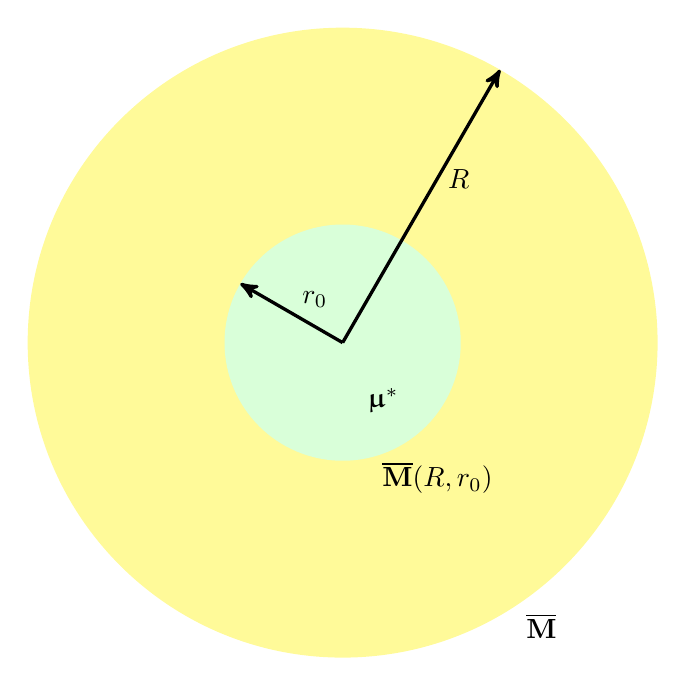
\begin{tikzpicture}
  \newcommand{\sz}{1cm}
  \newcommand{\szR}{4.0*\sz}
  \newcommand{\szr}{1.5*\sz}
  \fill[yellow!40!white] (0, 0) circle (\szR);
  \fill[green!15!white] (0, 0) circle (\szr);
  \draw[very thick, ->, >=stealth'] (0, 0) -- (60:\szR)
    node[pos=0.6, anchor=west]{$R$};
  \draw[very thick, ->, >=stealth'] (0, 0) -- (150:\szr)
    node[pos=0.5, anchor=210]{$r_0$};
  \node[] at (-55:0.6*\szr) {$\vmu^*$};
  \node[] at (-55:1.4*\szr) {$\vMbar(R, r_0)$};
  \node[] at (-55:1.1*\szR) {$\vMbar$};
\end{tikzpicture}
\end{center}



\subsection{Eq. (25) and the Green's theorem}



The Green's theorem mentioned before Eq. (25) is the following.
%
For a scale field $\psi$,
an integral over a region $v$
is equal to that over its surface $\vct S$:
\begin{equation}
  \int_v \nabla \psi \, d v
=
  \int_S \psi \, d\vct S,
  \label{eq:green}
\end{equation}
%
where the area element $d\vct S$
assumes the direction of the normal
and points out of the region.

The proof is the following (\cite{arfken}, chapter 1, \S 1.11).
%
The usual Gauss theorem states that
for a vector field $\vct F$,
\begin{equation}
  \int_v \nabla \cdot \vct F \, dv
=
  \int_S \vct F \vct \, d\vct S.
\end{equation}
%
Now let us use $\vct F = \psi \, \vct a$,
Since
\[
  \partial_i (a_i \psi)
= a_i \, \partial_i \psi
\]
we get that
\[
  \vct a \cdot \int_v \nabla \psi \, dv
=
  \vct a \int_S \vct F \vct \, d\vct S.
\]
Since $\vct a$ is arbitrary,
we get Eq. \eqref{eq:green}.

Applying this theorem to $\psi = -(\epsilon - 1) \, \psi_i$,
with the region between the two spheres
of radii $r_0$ and $R$,
we get
\begin{equation}
  \int_{v_0}^v \vP \, dv
=
  -\frac{\epsilon - 1}{4 \pi}
  \int^{S_e} \psi_i \, d\vct S
  +\frac{\epsilon - 1}{4 \pi}
  \int^{S_0} \psi_i \, d\vct S.
\end{equation}
Note,
\[
  4 \pi \, \vP
= (\epsilon - 1) \, \vE
= -(\epsilon - 1) \, \nabla \psi_i,
\]
in Gaussian units.



\subsection{Eq. (27)}



Equation (27) describes a uniform field within the $R$ ball.
\begin{equation}
  \chi
=
  \sum_{n = 1}^\infty
  \sum_{m = -n}^n
  B_{nm} r^n P_n^m(\cos\vartheta)e^{im \varphi}.
  \tag{27}
\end{equation}
%
Assuming that the dipole is along the $z$ axis,
this can be simplified using Legendre polynomials ($m = 0$) only
%
\begin{equation}
  \chi
=
  \sum_{n = 1}^\infty
  B_{n0} r^n P_n(\cos\vartheta).
  \tag{$27'$}
\end{equation}
%
In fact we will only need the $z = 1$ term,
\begin{equation}
  \chi
=
B_{10} \, r \cos\vartheta
=
B_{10} \, z,
  \tag{$27''$}
\end{equation}
%
which represents a uniform field within the $R$ ball.



\subsection{Eq. (28)}



The $\epsilon$ on the left-hand side of Eq. (28)
should be dropped:
\begin{align}
  -\vct\upmu^*\cdot
  \nabla
  \left(
    \frac { 1 }
    { |\vr - \vr'| }
  \right)
&=
  \sum_{n = 0}^\infty
  \sum_{m = -n}^{+n}
  \frac { ( n - |m| )! } { ( n + |m| )! }
  \notag
  \\
&\hphantom{=}\times
  \frac { A_{nm} } { r^{n + 1} }
  P_n^m(\cos\vartheta) e^{im \varphi}.
  \tag{28}
\end{align}
%
Again, if we can simplify this expression
by assuming that $\vmu^*$ aligns on the $z$ axis
$\vr' = \vct 0$, and keep the only relevant $n = 1$ term.
%
\begin{align}
  -\vct\upmu^*\cdot
  \nabla
  \left(
    \frac { 1 }
    { r }
  \right)
&=
  \frac { A_{10} } { r^2 }
  \cos\vartheta
=
  \frac { \mu_z^* } { r^2 }
  \cos\vartheta.
  \tag{$28''$}
\end{align}



\subsection{Eq. (30)}


Equations (30),
\begin{equation}
\begin{split}
  M_{nm}
&=
  \frac{ 2 n + 1 } { n \epsilon + n + 1 } A_{nm},
\\
  B_{nm}
&=
  \frac{ n + 1 }{ \epsilon R^{2 n + 1} }
  \frac{ \epsilon - 1 } { n \epsilon \epsilon + n + 1 }
  A_{nm}.
\end{split}
  \tag{30}
\end{equation}
%
are derived from the radial continuity of $\vct D$,
%
\begin{align*}
  \epsilon
  \left(
    \frac { n + 1 }{ \epsilon }
    \frac { A_{nm} } { R^{n+2} }
  - n B_{nm} R^{n - 1}
  \right)
=
  (n + 1) \frac{ M_{nm} }{ R^{n+2} },
\end{align*}
and the tangential continuity of $\vct E$,
\begin{align*}
  \frac { 1 }{ \epsilon }
  \frac { A_{nm} } { R^{n+1} }
+
  B_{nm} R^n
=
  \frac{ M_{nm} }{ R^{n+1} }.
\end{align*}



\subsection{Eq. (33)}



The term $\epsilon - 1$ in Eq. (33) misses a square sign.
\begin{align}
\vMbar
=
\vMbar(R, r_0)
-
\frac{2}{3\epsilon}
\frac{(\epsilon - 1)^2}{\epsilon + 2}
\vct\upmu^*
+ O\left( \frac{ r_0^3 } { R^3 } \right).
\tag{33}
\end{align}



\subsection{Definition of two dipole moments}



Both $\vmu^*$ and $\vMbar(R, r_0)$
Have the meaning of the total dipole of the region $v_0$
(within the sphere of the radius $r_0$).
%
However, from Eqs. (31) and (34), we get
\begin{equation}
  \vmu^* = \frac { 3 \epsilon } { 2 \epsilon + 1 }
  \vMbar(R, r_0) \ne \vMbar(R, r_0).
\end{equation}

It is should be noted that
$\vmu^*$ is simply the parameter
$A_{10}$ in (28)
and thus is not the physical dipole moment.
%
This is the parameter
that makes the region $v_0$
look like an effective dipole
immersed in the media of dielectric constant $\epsilon$.

Thus,
$\vmu^*$
contains some contribution of the polarization of the out sphere.
In fact
\begin{align*}
  \frac{ \vmu^* } { \epsilon }
&=
  \vMbar(R, r_0)
  -
  \frac { 2 (\epsilon - 1) } { 2 \epsilon + 1 } \vMbar(R, r_0).
  \\
&=
  \vMbar(R, r_0)
  -
  B_{10} R^3 \frac{ \epsilon + 2 }{ 3 }.
\end{align*}


\bibliography{../../liquid}
\bibliographystyle{alpha}
\end{document}
